\documentclass{sigchi}

% Use this section to set the ACM copyright statement (e.g. for
% preprints).  Consult the conference website for the camera-ready
% copyright statement.

% Copyright
\CopyrightYear{2020}
%\setcopyright{acmcopyright}
\setcopyright{acmlicensed}
%\setcopyright{rightsretained}
%\setcopyright{usgov}
%\setcopyright{usgovmixed}
%\setcopyright{cagov}
%\setcopyright{cagovmixed}
% DOI
\doi{https://doi.org/10.1145/3313831.XXXXXXX}
% ISBN
\isbn{978-1-4503-6708-0/20/04}
%Conference
\conferenceinfo{CHI'20,}{April  25--30, 2020, Honolulu, HI, USA}
%Price
\acmPrice{\$15.00}

% Use this command to override the default ACM copyright statement
% (e.g. for preprints).  Consult the conference website for the
% camera-ready copyright statement.

%% HOW TO OVERRIDE THE DEFAULT COPYRIGHT STRIP --
%% Please note you need to make sure the copy for your specific
%% license is used here!
% \toappear{
% Permission to make digital or hard copies of all or part of this work
% for personal or classroom use is granted without fee provided that
% copies are not made or distributed for profit or commercial advantage
% and that copies bear this notice and the full citation on the first
% page. Copyrights for components of this work owned by others than ACM
% must be honored. Abstracting with credit is permitted. To copy
% otherwise, or republish, to post on servers or to redistribute to
% lists, requires prior specific permission and/or a fee. Request
% permissions from \href{mailto:Permissions@acm.org}{Permissions@acm.org}. \\
% \emph{CHI '16},  May 07--12, 2016, San Jose, CA, USA \\
% ACM xxx-x-xxxx-xxxx-x/xx/xx\ldots \$15.00 \\
% DOI: \url{http://dx.doi.org/xx.xxxx/xxxxxxx.xxxxxxx}
% }

% Arabic page numbers for submission.  Remove this line to eliminate
% page numbers for the camera ready copy
% \pagenumbering{arabic}

% Load basic packages
\usepackage{balance}       % to better equalize the last page
\usepackage{graphics}      % for EPS, load graphicx instead 
\usepackage[T1]{fontenc}   % for umlauts and other diaeresis
\usepackage{txfonts}
\usepackage{mathptmx}
\usepackage[pdflang={en-US},pdftex]{hyperref}
\usepackage{color}
\usepackage{booktabs}
\usepackage{textcomp}

% Some optional stuff you might like/need.
\usepackage{microtype}        % Improved Tracking and Kerning
% \usepackage[all]{hypcap}    % Fixes bug in hyperref caption linking
\usepackage{ccicons}          % Cite your images correctly!
% \usepackage[utf8]{inputenc} % for a UTF8 editor only

% If you want to use todo notes, marginpars etc. during creation of
% your draft document, you have to enable the "chi_draft" option for
% the document class. To do this, change the very first line to:
% "\documentclass[chi_draft]{sigchi}". You can then place todo notes
% by using the "\todo{...}"  command. Make sure to disable the draft
% option again before submitting your final document.
\usepackage{todonotes}

% Paper metadata (use plain text, for PDF inclusion and later
% re-using, if desired).  Use \emtpyauthor when submitting for review
% so you remain anonymous.
\def\plaintitle{Individual Plan - Degree Project}
\def\subplaintitle{
  Reducing Sedentary Behavior for Software Engineers: Identified Performance Advantages and Disadvantages Using a Visual Programming Language Inside Virtual Reality}
\def\plainauthor{First Author, Second Author, Third Author,
  Fourth Author, Fifth Author, Sixth Author}
\def\emptyauthor{}
\def\plainkeywords{Authors' choice; of terms; separated; by
  semicolons; include commas, within terms only; this section is required.}
\def\plaingeneralterms{Documentation, Standardization}

% llt: Define a global style for URLs, rather that the default one
\makeatletter
\def\url@leostyle{%
  \@ifundefined{selectfont}{
    \def\UrlFont{\sf}
  }{
    \def\UrlFont{\small\bf\ttfamily}
  }}
\makeatother
\urlstyle{leo}

% To make various LaTeX processors do the right thing with page size.
\def\pprw{8.5in}
\def\pprh{11in}
\special{papersize=\pprw,\pprh}
\setlength{\paperwidth}{\pprw}
\setlength{\paperheight}{\pprh}
\setlength{\pdfpagewidth}{\pprw}
\setlength{\pdfpageheight}{\pprh}

% Make sure hyperref comes last of your loaded packages, to give it a
% fighting chance of not being over-written, since its job is to
% redefine many LaTeX commands.
\definecolor{linkColor}{RGB}{6,125,233}
\hypersetup{%
  pdftitle={\plaintitle},
% Use \plainauthor for final version.
%  pdfauthor={\plainauthor},
  pdfauthor={\emptyauthor},
  pdfkeywords={\plainkeywords},
  pdfdisplaydoctitle=true, % For Accessibility
  bookmarksnumbered,
  pdfstartview={FitH},
  colorlinks,
  citecolor=black,
  filecolor=black,
  linkcolor=black,
  urlcolor=linkColor,
  breaklinks=true,
  hypertexnames=false
}

% create a shortcut to typeset table headings
% \newcommand\tabhead[1]{\small\textbf{#1}}

% End of preamble. Here it comes the document.
\begin{document}

\title{%
  \plaintitle \\
  \large \subplaintitle
}

\numberofauthors{3}
\author{
  \alignauthor{Adam Jonsson\\
  \affaddr{Stockholm, Sweden}\\
  \email{adajon@kth.se}}\\
}

\maketitle


% ACM Classfication

\begin{CCSXML}
<ccs2012>
<concept>
<concept_id>10003120.10003121</concept_id>
<concept_desc>Human-centered computing~Human computer interaction (HCI)</concept_desc>
<concept_significance>500</concept_significance>
</concept>
<concept>
<concept_id>10003120.10003121.10003125.10011752</concept_id>
<concept_desc>Human-centered computing~Haptic devices</concept_desc>
<concept_significance>300</concept_significance>
</concept>
<concept>
<concept_id>10003120.10003121.10003122.10003334</concept_id>
<concept_desc>Human-centered computing~User studies</concept_desc>
<concept_significance>100</concept_significance>
</concept>
</ccs2012>
\end{CCSXML}

\ccsdesc[500]{Human-centered computing~Human computer interaction (HCI)}
\ccsdesc[300]{Human-centered computing~Haptic devices}
\ccsdesc[100]{Human-centered computing~User studies}

\section{Project Information}

\subsubsection{Preliminary title}
\subplaintitle.

\subsubsection{Student} 
Adam Jonsson - adajon@kth.se

\subsubsection{Examiner} 
Cristian Bogdan - cristi@kth.se

\subsubsection{Supervisor} 
Martin Hedlund - marthed@kth.se

\subsubsection{Current Date} 
2022-01-11

\subsubsection{Keywords} 
Visual Programming Language, Virtual Reality, Performance, Health.

\section{Background And Objective}

Professions that are primarily conducted sedentary have increased due to the growth of office-related occupation \cite{parry_contribution_2013}. One such profession is software engineering. A concern with this direction is that sedentary behavior has been found to have a negative effect on a person's health, such as obesity \cite{lakdawalla_labor_2007}, depression \cite{zhai_sedentary_2015}, and a higher risk of cardiovascular events \cite{straker_sedentary_2016}. Therefore, it is of interest to reduce sedentary, making the work environment healthier.

There exist previous studies exploring ways to prevent sedentary behavior during work, such as making the employers more aware of their activity with the help of notification from a mobile application \cite{cole_they_2015}, introducing standing desks \cite{pronk_reducing_2012}, and walking while having meetings \cite{bort-roig_uptake_2014}. One of these studies found that to make the change be of effect, the intervention can not hurt the productivity and needs to be customized for the work context \cite{bort-roig_uptake_2014}.

% Similarly, this degree project aims to explore the potential to reduce the sedentary behavior for software engineers. But instead of adding intervention to the work environment, this study explores the potential of conducting software engineering in virtual reality that requires movement, reducing the sedentary behavior form the work itself.

Another potential means of reducing sedentary behavior is using virtual reality (VR) during work. This is because a VR device that uses six degrees of freedom has its benefit in that it requires more movement than sitting in front of a computer. A typical VR application might need users to walk, look around, and move their arms to grab or push interactable. Of course, the design of a VR application heavily affects the frequency at which these movements occur. Compare this to a mouse and keyboard setup, where the user only needs to do small movements with their fingers and wrist to interact with a GUI. One meta-analysis on physical training in VR concluded that the technology has potential \cite{ng_effectiveness_2019}

While VR can be beneficial in increasing movement, one potential issue with conducting software engineering inside VR is the performance. Software engineering as an occupation often requires programming, which is typically done with the help of a keyboard. One study has found that many typing technics with VR controllers are significantly slower compared to using a qwerty keyboard \cite{speicher_selection-based_2018}. Therefore, generating code by typing inside VR might prevent sedentary behavior but potentially reduce productivity.

\begin{figure}[h]
  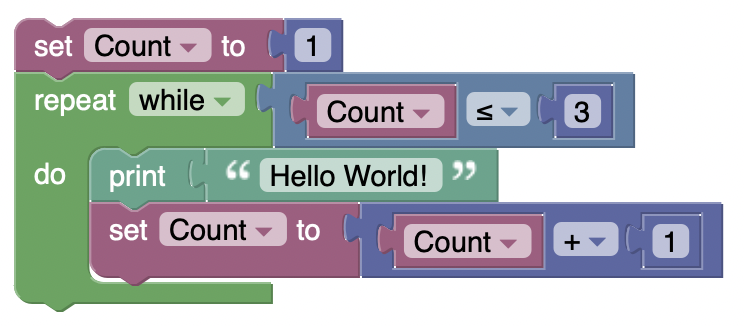
\includegraphics[width=\linewidth]{figures/blockly.png}
  \caption{Example of code inside Blockly}
  \label{fig:blockly}
\end{figure}

% Change this & fix references
One approach that does not primarily requires text entry input is using a visual programming language (VPL). That is, one needs to move elements around in a program in order to create the desired outcome. There are mainly two types of VPL. One is a block-based approach, similar to putting lego together, which is forcing a specific layout of the code blocks \cite{mason_block-based_2017}. The other is a flow-based approach which is more like putting cables together and is instead more free regarding placement of the code \cite{mason_block-based_2017}. Blockly is a popular block-based open source VPL published by Google and has been shown to be easy to understand and get started with \cite{seraj_scratch_2019}, see figure \ref{fig:blockly}. Blockly is built using code blocks, each block representing a type of code. The green one seen in figure \ref{fig:blockly} is, for example, a while loop, while the light blue is a logic comparator.

VPLs have previously been implemented in VR. For example, FlowMatic \cite{zhang_flowmatic_2020} is a flow-based environment for creating VR applications, while Cubely \cite{vincur_cubely_2017} makes use of blocks for teaching programming. HackVR \cite{kao_hackvr_2020} combines the flow-based approach with the object-oriented paradigm. However, none of these studies focused on the health aspect or compared the performance of doing a VPL in front of a computer.

However, a potential challenge in making a VPL inside VR that is both performant and contributes to movement is that those two factors might work against each other. That is, the more movement the application requires, the less performant it will be, and vice versa. For example, having interactable objects further apart from each other will make the user need to move more. However, it will hurt productivity as the user needs to move forth and back, as compared to them having them close together. A VPL inside VR might have such issues depending on its design. However, there are types of interactions in a VPL inside VR other than walking, such as connecting code blocks, restructuring current, and navigating around the code space. These other interactions may have movement/performance relationships that differ from moving between points A and B. Not knowing these relationships or performance differences can make designing a VPL in VR challenging. Therefore, identifying these relationships and comparing the performance to doing VPL on a computer can help accelerate the development of a performant VPL inside VR. Which in turn can be used to reduce sedentary behavior for software engineers.

To conclude, in this degree project, the potential of reducing sedentary behavior for software engineering using virtual reality will be explored. More specifically, performance differences in relation to movement between coding in a VPL inside virtual reality and a computer will be measured. This degree project aims to contribute to future researchers and designers in creating an efficient visual programing language inside virtual reality that can reduce sedentary behavior while also being performant.

\section{RESEARCH QUESTION AND METHOD}

\subsection{Question}
The main research question that is going to be explored in this degree project is as follows:

\textit{
  "What are the performance differences in relation to movement between coding using a visual programming language inside virtual reality and a computer?"
}

One potential outcome could be that the performance and movement differences reside in different areas of working with a VPL. For example, say that working with a VPL is divided into three categories: 1) connecting code blocks, 2) adding new code blocks using a menu, and 3) moving and restructuring existing blocks. Because VR and computers usually have different input and output modalities, some categories could differ depending on the platform used. Connecting code block may be faster using VR as both hands can be used, while only the mouse can be used on a computer. However, using the menu may be faster on a computer while slower on VR, possibly due to the VR use requiring more movement than a computer. These findings may help designers and researchers decide what interactions need to be improved or changed altogether to make VPL in VR work. 

\subsection{Objectives}
As previously mentioned, the main objective of this degree project is to create a paper to help future researchers and designers to create a performant VPL inside VR that can reduce sedentary behavior for software engineers. In order to make the report as giving as possible, the following objectives need to be reached.

\begin{itemize}
  \item Identify how areas of coding in a VPL differ in terms of performance and movement.
  \item Explore the correlation between the tracked movement and performance.
  \item Discuss how the design differences potentially contribute to the observed data.
\end{itemize}

\subsection{Tasks}
To research the above mentioned objects, the followings tasks needs to be completed:

\subsubsection{Create a VPL inside VR}
A VPL inside VR needs to be created based on an existing VPL design for traditional 2D GUI. No existing VPL in VR is used, as the design can vary between the one used in VR and the one used on a computer. In this case, the movement and performance differences may be influenced more by the design rather than the platform it is used on. For this reason, creating a VPL for VR based on an existing VPL for a computer will ensure that the design differences are to the minimum. Blockly is currently the top candidate to base the VPL on, as it is simple and has a public API with good documentation.

\subsubsection{Find a method to measure performance and movement}
A method of gathering movement and performance data needs to be explored and implemented in both the VR and the computer platform. However, this study can use previous research about movement when sitting in front of a computer instead of doing body tracking. The reason is that movement is assumed to be similar for most computer-related tasks. Regarding VR movement tracking, a challenge is that the sample rate should be relatively high to reduce the amount of error in the accumulated distance moved. This will result in a large data set that needs to be stored and analyzed. Therefore, it can be helpful to check whether the data gathering is technically possible early in the project. 

\subsubsection{Categories interactions of a VPL}
To get a more detailed comparison between working with a VPL in VR and a computer, the interaction with a VPL should be categorized into different areas. This allows one to compare movement and performance for each individual area. For example, the observed performance and movement while connecting blocks or moving blocks might differ depending on the platform used. Thus, giving a better insight into the differences. The challenge here is to create categories that are easy to identify for both VR and a computer.

\subsubsection{Create programming tasks}
Programming tasks need to be created to gather data about the movement and performance. The programing tasks should have a difficult level such that it takes about one minute to figure out the solution. This minimizes the time spent thinking about the task and maximizes the time to implement the solution in code. However, this is a challenge as the perceived difficulty level may vary between participants. Moreover, figuring out the solution may also occur while coding. For these reasons, variation needs to be allowed to happen and mentioned as a limitation in this study.

\subsubsection{Create a tutorial}
Because a number of participants may have limited experience of using VR, a steep learning curve will be present when the participants first use the VR headset. This learning curve will probably revolve around learning the controllers and moving around in the virtual world. In order to prevent this learning curve from affecting the result, a tutorial of the basic controls and logic should be created.

\subsection{Method}
The method can be divided into three stages: 1) Information and conditions of participating, 2) Data gathering, and 3) Data analysis. Each stage is described in more detail below:

\subsubsection{Information and conditions of participating}
For each potential participant, information regarding data management and the possibility to withdraw at any moment needs to be communicated before the study starts. The possibility of quitting participating is important as there is a change of the participants feeling simulation sickness during the experiment.

\subsubsection{Data gathering}
Participants' body measurements and previous experience with VR, VPL, and JavaScript are gathered by filling in a created form. This data is used for the metabolic equivalent of task (METs) calculations to see if previous experience correlates to the participants' performance. The observed METs can be used to compare the movement in VR to other physical activities, such as sitting still, standing, and walking.

In order to gather and compare performance data, each participant is to solve several programming tasks three times, each time using a different platform. These platforms are text entry programming, a VPL using a computer, and a VPL using VR. The programming tasks are identical for every platform used. The time it takes the participant to complete every task is documented by recording the screen. However, the participants will presumably be more performant each time they solve the same programming tasks. For this reason, half of the participants will do the VPL using a computer before doing a VPL inside VR. The other half does the opposite. All participants will start with the text entry coding to create a baseline to compare the performance and movement. This method will result in two comparison groups, those participants that used the VPL inside VR or computer the first time and those who did it the second time. Furthermore, differences can be observed within the two groups to get an insight into the learning curve's effect on the participants' performance.

Before and after using the VR headset, the user answers a simulation sickness questionnaire to identify potential factors that could affect the observed result. Moreover, a tutorial for the VPL inside VR and the computer needs to be completed before the participants start with the programming tasks. This is to reduce the effect of the learning curve for the basics around VPL and the controls.

\subsubsection{Data analysis}
Different types of interaction with the VPL are going to be categorized, such as connecting code blocks, removing code blocks, adding code blocks, being stationary, etc. These categories are used to do a more detailed comparison between the VPL inside VR and on a computer. Screen recordings of the participants using the VPL in both platforms are coded into these specified categories. After which, the time spent and the tracked movement are compared between the different categories by using mean and standard divination. More complex statistics, such as a t-test, can be used if the number of participants is enough.

% \subsection{Ethics and Sustainability}
% Does the project address questions of ethics or sustainability? Does the project raise ethical or sustainability questions? If yes, how could these be handled?

\subsection{Limitations}
This study focuses on one aspect of programming in a VPL, which is to generate relatively small pieces of code that solves a simple problem. There are many other aspects to programming, such as debugging, refactoring, testing, etc. However, while the mentioned aspect is important for future research, these aspects are out of this degree project's scope. Moreover, the study is limited to exploring the differences between using a block-based VPL based on an existing design called Blockly. Thus, the result does not reflect the full potential of a VPL inside VR but rather sheds light on potential issues and benefits of designing a VPL based on an existing VPL for two-dimensional GUIs.

\subsection{Risks}
Due to the COVID-19 situation, acquiring participants willing to use a VR headset can be challenging. The risk is that too few volunteers are found, making the result of this study inconclusive. In order to minimize this risk, health information such as the headset being sanitized after every use is communicated. Moreover, a reward for participating could also increase the number of volunteers. 

Another risk is development roadblocks. There is a chance that bugs and challenging implementation are discovered late into the project development. This will also potentially make the result inconclusive. For this reason, development is going to be worked on early into the project, creating first a minimal viable product (MVP). Having an MVP is insurance that every aspect of this study is technically possible. Thus, roadblocks will probably occur early, and alternations to the project can be made without postponing the deadline.

\section{EVALUATION AND NEWS VALUE}
This degree project's objective is to explore the differences in performance in relation to movement between coding using a VPL inside VR and on a computer. The objective is reached when enough movement and performance data has been gathered and analyzed such that conclusions can be made. Examples of such conclusions can be that connecting blocks have the same performance in VR as on a computer and comprise 30 percent of the total movement. This shows that there is potential to use this interactive method. However, interacting with the menu might be less performant and only comprise 10 percent of the total movement,  indicating that this interaction needs to be improved or changed.

The news value of this research is to give a broad view of the movement advantages in relation to potential performance disadvantages using a VPL inside VR. Designers can use the result to make design decisions or see if VR is a viable technology for VPLs. Researchers can potentially use the result to identify interesting research areas.

\section{PRE-STUDY}
The literature review will consist of existing research surrounding the topic of reducing sedentary behavior. Background on VPL will also be studied, including existing VPLs inside VR. HackVR, FlowMatic, and Cubely are some of the existing VPLs using VR that currently have been found. Furthermore, VR overall will be researched, such as the typical benefits and downside of using it. Also, the current design recommendation for VR will be reviewed and applied when designing the VPL implementation in VR. Lastly, ways to compute estimated METs from movement data will be researched. While it is not essential, it will make the movement data more graspable as it can be compared to other types of activities.

\section{CONDITIONS AND SCHEDULE}
In order to conduct the experiment described in the suggested methodology, the following equipment needs to exist: A VR headset with six degrees of freedom, a room that is at least has 5x5 meter space, and a computer. For the interview subject, all need to have some experience with programming because programming tasks need to be completed. Previous experience with VR or VPL is allowed to vary between participants.

The supervisor is to guide and give recommendations throughout the entire degree project. This is by having recurring meetings where progress is reported, and feedback is given from the supervisor. Moreover, because the supervisor is currently working around the same research area, sharing useful literature with each other can also be expected.

The schedule is presented in weeks. However, note that this is a preliminary planing and may change in the future:

\begin{itemize}
  \item \textbf{W5 - Literature Review \& Development.} Research existing prevention for sedentary behavior during work. Basic development for VPL inside VR.
  \item \textbf{W6 - Literature Review \& Development.} Research existing VPLs, their performance compared to typical programming and other differences. Basic development for VPL inside VR.
  \item \textbf{W7 - Literature Review \& Development.} Research VR, both in terms of design recommendation as well as movement tracking. Basic development for VPL inside VR.
  \item \textbf{W8 - Literature Review \& Development.} Research existing VPL inside VR . Basic development for VPL inside VR.
  \item \textbf{ END OF W8 MILESTONE  } - Literature review done and the core logic for the VPL inside VR works.
  \item \textbf{W9 - Design \& Development.} - Choose design for the VPL inside VR from the litteratur found. Document every design difference between the VPL in VR and on a computer.
  \item \textbf{W10 - Design \& Development.} - Implement the chosen design into the VPL in VR.
  \item \textbf{W11 - Design \& Development.} - Develop the VPL such that code can be generated and shown in VR. 
  \item \textbf{W12 - Design \& Development.} - Develop the ability to complete programming tasks on all platforms.
  \item \textbf{W13 - Design \& Development.} - Create tutorial for VPL inside VR and on a computer.
  \item \textbf{W14 - Design \& Development.} - Create programming tasks and make sure that they can be solved on all platforms.
  \item \textbf{ END OF W14 MILESTONE  } - VPL inside VR is functional and code can be created with it.
  \item \textbf{W15 - Movement Tracking \& Development.} - Investigate and implement method of tracking movement with VR.
  \item \textbf{W16 - Pilot Study.} - Create all questionnaires and conduct a pilot test to check if everything works and that data can be gathered as planed.
  \item \textbf{ END OF W16 MILESTONE  } - VPL for all platforms are ready and data gathering can start.
  \item \textbf{W17 - Data Gathering } - Invite participants and start gathering data.
  \item \textbf{W18 - Data Gathering } - Continue inviting participants and  gathering data.
  \item \textbf{W19 - Data Analysis} - Categorize interaction types from video recordings and make statistical analyzes on the gathered data.
  \item \textbf{ END OF W19 MILESTONE } - Data is fully gathered.
  \item \textbf{W20 - Writing } - Write about the analyzed data.
  \item \textbf{W21 - Writing } - Refine paper.
  \item \textbf{W22 - Writing } - Refine paper.
  \item \textbf{W23 - Writing } - Refine paper.
  \item \textbf{W24 - Writing } - Prepare final presentation.

\end{itemize}

% REFERENCES FORMAT
% References must be the same font size as other body text.
\bibliographystyle{SIGCHI-Reference-Format}
\bibliography{References}

\end{document}

%%% Local Variables:
%%% mode: latex
%%% TeX-master: t
%%% End:
